\documentclass[14pt]{article}

\usepackage[utf8x]{inputenc}
\usepackage[russian]{babel}
\usepackage{graphicx}
\usepackage{caption}
\usepackage{float}
\graphicspath{{images/}}
\DeclareGraphicsExtensions{.pdf,.png,.jpg}

\usepackage{amsmath}
\usepackage{pgfplots}

\usepackage{geometry} % Меняем поля страницы
\geometry{left=2cm}% левое поле
\geometry{right=1.5cm}% правое поле
\geometry{top=2cm}% верхнее поле
\geometry{bottom=2cm}% нижнее поле

\renewcommand{\theenumi}{\arabic{enumi}}
\renewcommand{\labelenumi}{\arabic{enumi}}
\renewcommand{\theenumii}{.\arabic{enumii}}
\renewcommand{\labelenumii}{\arabic{enumi}.\arabic{enumii}.}
\renewcommand{\theenumiii}{.\arabic{enumiii}}
\renewcommand{\labelenumiii}{\arabic{enumi}.\arabic{enumii}.\arabic{enumiii}.}

\begin{document}
\begin{titlepage}
	\begin{center}
		\fontsize{18pt}{20pt}\selectfont
		\textbf{Работа 4.3.3.}	
	
		\vspace{5cm}
		\fontsize{24pt}{25pt}\selectfont
		Исследование разрешающей способности микроскопа методом Аббе
	\end{center}
	\begin{flushright}
		\fontsize{18pt}{20pt}\selectfont
		\vspace{14cm}
		\hspace{-3cm}
		\textit{Корнеев Е.С.}
	\end{flushright}		
\end{titlepage}

\begin{center}
	\fontsize{16pt}{18pt}\selectfont	
	Исследование разрешающей способности микроскопа методом Аббе
\end{center}


\fontsize{14pt}{16pt}\selectfont
\vspace{1cm}
\textbf{Цель работы:} изучение дифракционного предела разрешения объектива микроскопа.

\vspace{0.5cm}
\textbf{Оборудование:} лазер; кассета с набором сеток разного
периода; линзы; щель с микрометрическим винтом; оптический стол
c набором рейтеров и крепёжных винтов; экран; линейка.

\vspace{1cm}

Всякая оптическая система, предназначенная для получения изображений,
имеет конечный предел разрешения, т. е. ограниченную возможность
раздельного наблюдения близких частей предмета. Принципиальной
причиной, ограничивающей предел разрешения, является дифракция
световых волн: ограничение пучка лучей краями линз и диафрагм,
составляющих оптическую систему, приводит к нарушению \textsl{стигматичности}
изображения — каждая точка предмета отображается не в одну
точку, а в дифракционное пятно. Дифракционные пятна от близких точек
предмета могут перекрываться друг другом, в результате чего точки
становятся неразличимыми.

\textsl{Разрешающей способностью оптического прибора} называют минимальное
расстояние lmin между двумя точками в пространстве предметов,
изображения которых разрешаются по критерию Релея.

Природа дифракционных искажений общая для всех оптических систем;
мы рассмотрим для примера глаз, лупу и простейший объектив
микроскопа, состоящий из одной линзы (разрешение оптических приборов
определяется обычно дифракцией на объективе).
Оценим разрешающую способность глаза, полагая, что предмет
(рис. 1) расположен на расстоянии наилучшего зрения $L = 25$ см от
зрачка диаметром $d_0$ = 5 мм. Согласно критерию Релея глаз различает
изображение точек как два объекта, если угловое расстояние между
точками соответствует угловому размеру дифракционного пятна:
$$
	\frac{l_\text{min}}{L} = \frac{\lambda}{d_0}
$$

или
$$
	l_\text{min} = \lambda\frac{L}{d_0} \approx \lambda\frac{25}{0.5} = \approx 50\lambda
$$

\begin{figure}[h!]
	\center{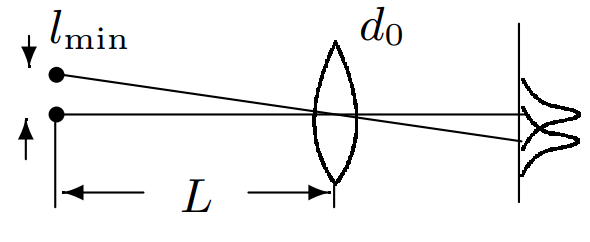
\includegraphics[width = 8cm]{1}}
	\caption{Разрешающая способность глаза}
	\label{fig:image}
\end{figure}

Для лупы диаметром $D_0$ с фокусным расстоянием $f$ при настройке
глаза на бесконечность
$$
	l_\text{min} = \lambda\frac{f}{D_0}
$$

Для иммерсионного микроскопа (объект находится в иммерсионной
среде -- жидкости с показателем преломления n) разрешающая способность объектива
$$
	l_\text{min} \approx \frac{0.61\lambda}{n\sin u} \approx \frac{\lambda}{2n\sin u},
$$
\noindent где $u$ -- апертурный угол объектива микроскопа (см. рис. 2), т. е. угол
между оптической осью
и лучом, направленным из центра объекта
в край линзы (напомним, что при наблюдении в микроскоп объект занимает
небольшой участок, располагающийся вблизи оптической оси объектива).

\begin{figure}[h!]
	\center{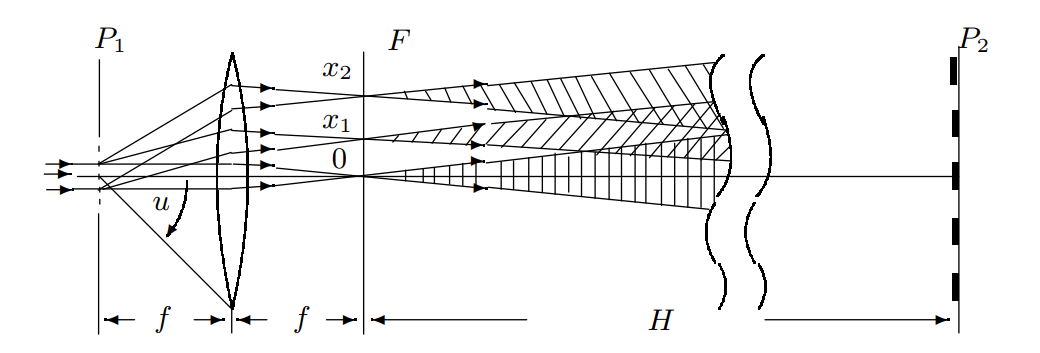
\includegraphics[width = 15cm]{2}}
	\caption{Образование изображения в объективе микроскопа. $P_1$ -- плоскость предмета, $F$ -- задняя фокальная плоскость объектива,
			 $P_2$ -- плоскость, сопряженная с предметной плоскостью. В плоскости $P_2$ световые пучки сильно перекрываются}
	\label{fig:image}
\end{figure}

Если наблюдения с помощью микроскопа ведутся при внешнем освещении, то,
как правило, различные точки предмета рассеивают когерентные волны.
Теория разрешающей способности для случая освещаемых
объектов была разработана Аббе.

Схема образования изображения в объективе микроскопа представлена
на рис. 2. Для простоты рассмотрим случай, когда предметом является периодическая структура 
(дифракционная решетка), освещаемая параллельным пучком лучей. При наблюдении в микроскоп
предмет располагается вблизи переднего фокуса объектива.

Аббе предложил иной подход к оценке разрешающей способности: про
хождение лучей от предмета к изображению разбивается на два этапа.
Сначала рассматривается картина, возникающая в задней фокальной
плоскости $F$ объектива. Эта картина называется \textsl{первичным изображением}
или \textsl{фурье-образом} предмета. Затем первичное изображение
рассматривается как источник волн, создающих изображение предмета
в плоскости $P_2$, сопряженной плоскости предмета, т. е. \textsl{вторичное изображение}.
Такой подход основан на \textsl{принципе Гюйгенса-Френеля}, согласно
которому любой участок волнового фронта можно рассматривать
как вторичный источник излучения.

Легко понять, что первичное изображение, наблюдаемое в задней фокальной
плоскости объектива, представляет собой картину дифракции Фраунгофера на объекте (в нашем случае
-- на дифракционной решетке).
Действительно, на решетку падает плоская волна, а
каждая точка наблюдения в фокальной плоскости $F$ линзы соответствует бесконечно
удаленной точке. Смещение $x_m$ точки наблюдения от оптической оси
связано с углом наклона $\varphi_m$ параллельного пучка лучей перед линзой
соотношением (при малых $\varphi$): $x_m \approx f\varphi_m$.

\begin{figure}[h!]
	\center{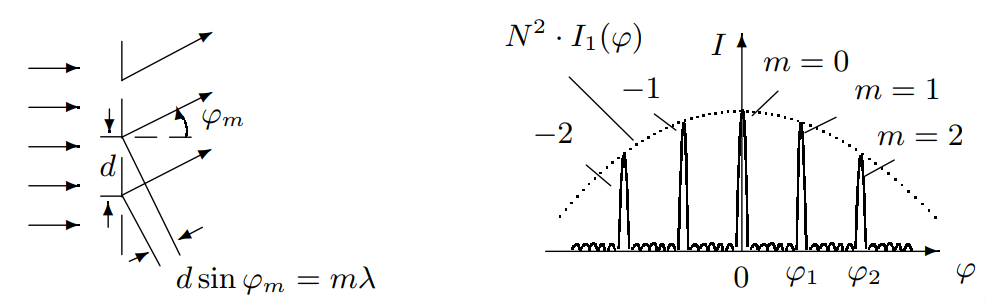
\includegraphics[width = 15cm]{3}}
	\caption{Спектр амплитудной решетки. $I_1(\varphi)$ -- распределение интенсивности при дифракции света на одиночной щели, $N$ -- число щелей решетки}
	\label{fig:image}
\end{figure}

При дифракции Фраунгофера на одномерной решетке периода
$d$ направления $\varphi_m$ максимальной интенсивности (главные максимумы) определяются
условием:
\begin{equation}
	d\sin\varphi_m = m\lambda
\end{equation}
\noindent где $\lambda$ -- длина световой волны. Главные максимумы различных порядков
$m$ имеют неодинаковые интенсивности (рис. 3). Таким образом,
первичное изображение представляет собой набор ярких точек, расположенных цепочкой на равных
расстояниях друг от друга. Излучение этих когерентных точечных источников создаст в плоскости
$P_2$ систему интерференционных полос, синтезирующих изображение предмета (решетки)
в этой плоскости.

При таком рассмотрении дифракционные искажения, обусловленные
конечным диаметром линзы, связаны с тем, что часть первичного изображения
закрывается. Через микроскоп проходят только те пучки, для
которых выполняется условие
\begin{equation}
	\varphi_m < u
\end{equation}
\noindent где $u$ -- \textsl{апертурный угол} (рис. 2). Эти пучки лучей собираются в задней
фокальной плоскости линзы, так что за ней возникают расходящиеся пучки лучей с центрами в плоскости
$F$. В плоскости $P_2$ эти пучки интерферируют и воспроизводят увеличенное изображение решетки.

Из рис. 2 ясно, что диафрагмы практически одинаковых размеров, расположенные в фокальной плоскости
$F$ или непосредственно на объективе, перекрывают те же самые пучки лучей.
Таким образом, дифракцию на оправе объектива в рассмотрении Аббе можно заменить дифракцией
на диафрагме $D$, равной по размеру диаметру работающей (открытой)
части линзы и расположенной в задней фокальной плоскости $F$.

Рассмотрим вначале крайний случай, когда через диафрагму в плоскости
$F$ проходит только один максимум -- максимум нулевого порядка.
Картина в $P_2$ изображает при этом объект, первичное изображение которого
сводится к одному центральному максимуму. Но такая картина возникает лишь в том случае,
когда параллельный пучок не претерпевает никакой дифракции, т е. если решетка вообще отсутствует;
в плоскости $P_2$ получается поэтому равномерное распределение освещенности
и решетка не видна.

Если приоткрыть диафрагму и поставить ее несимметрично, так, чтобы
прошел только нулевой и один из первых максимумов, то на экране
получится изображение, имеющее вид периодической структуры с плавным
переходом от светлых мест к темным; такое изображение
характерно для двухлучевой интерференции. Рассчитаем период изображения в
плоскости $P_2$ для этого случая. Линейное расстояние $x_1$ между максимумами
нулевогои первого порядка в плоскости $F$ есть
\begin{equation}
	x_1 = f\varphi_1 = f\lambda/d
\end{equation}

Ширина $l$ интерференционных полос, образующихся в плоскости $P_2$, может
быть найдена по формуле
\begin{equation}
	l = \lambda/\omega,
\end{equation}
\noindent где $\omega = x_1/H$ -- угол схождения интерферирующих лучей в точке наблюдения,
расположенной в плоскости $P_2$, а $H$ -- расстояние между плоскостями $F$ и $P_2$. Таким образом,
\begin{equation}
	l \approx \lambda H/x_1 = Hd/f.
\end{equation}

Согласно геометрической оптике изображение решетки в плоскости
$P_2$ должно иметь период
\begin{equation}
	d' \approx \frac{H + f}{f}d
\end{equation}

Поскольку в случае микроскопа предмет располагается вблизи передней
фокальной плоскости объектива, и, следовательно, $H \ll f$, получаем:
$l \approx d'$. Таким образом, с помощью дифракционных максимумов нулевого
и первого порядка в увеличенном масштабе передается основной период решетки
(и не воспроизводятся никакие детали структуры, например, наличие резкой границы между светлыми
и темными участками дифракционной решетки).

Если задержать каким-либо образом в плоскости $F$ максимум первого
порядка, а вместо него пропустить максимум второго порядка, то
в $P_2$ возникнет система полос с периодом в два раза меньшим, так что
на экране будет видно изображение более частой решетки, чем имеющаяся в действительности. 
Максимумы высших порядков создают более узкие интерференционные полосы, они ответственны за передачу более
тонких деталей.

Из изложенного ясно, что для получения правильного изображения
надо, чтобы через объектив микроскопа проходили дифракционные пучки
разных направлений. Как уже отмечалось ранее, если апертурный угол
$u$ меньше $\varphi_1$, то в плоскости $P_2$ не возникает периодического изображения.
Соотношение
\begin{equation}
	\sin u \geq \lambda/d
\end{equation}
\noindent можно рассматривать как условие разрешения решетки с периодом
$d$. Отсюда можно найти минимальное разрешаемое объективом расстояние
\begin{equation}
	d \geq \frac{\lambda}{\sin u} \approx \frac{\lambda}{(D/2f)}.
\end{equation}

При этом диафрагма $D$, расположенная симметрично, пропускает нулевой и
$\pm 1$ максимумы.

При освещении решётки пучками, наклонными к оси,
когда через диафрагму, кроме нулевого, проходит всего один из двух первых максимумов
(этого достаточно для изображения периодической структуры без тонких деталей),
условие разрешения принимает вид
$$
	d \geq \frac{\lambda}{2\sin u}.
$$

В нашей работе применяется двумерная решетка -- сетка. Ее можно рассматривать
как две скрещенные (перпендикулярные друг к другу) решетки. Узкий пучок монохроматического света,
пройдя через решетку с вертикальными штрихами, дает совокупность максимумов, расположенных
вдоль горизонтальной линии. Световой пучок, соответствующий каждому максимуму, про
ходя через вторую решетку, распадается на новую совокупность световых пучков, дающих максимумы
вдоль вертикальной линии. Главные максимумы возникают тогда, когда одновременно
выполняются условия:
\begin{equation}
	d\sin\varphi_x = m_x\lambda,~~~d\sin\varphi_y = m_y\lambda
\end{equation}
\noindent где $m_x$ и $m_y$ -- целые числа, характеризующие порядки дифракционных
максимумов, $\varphi_x$ и $\varphi_y$ -- направления на главные дифракционные максимумы
в горизонтальной и вертикальной плоскостях соответственно.

Максимумы, удовлетворяющие условию $\varphi_x, \varphi_y < u$, создают в задней фокальной плоскости
$F$ объектива картину дифракции Фраунгофера (рис. 4) -- первичное изображение.

\begin{figure}[h!]
	\center{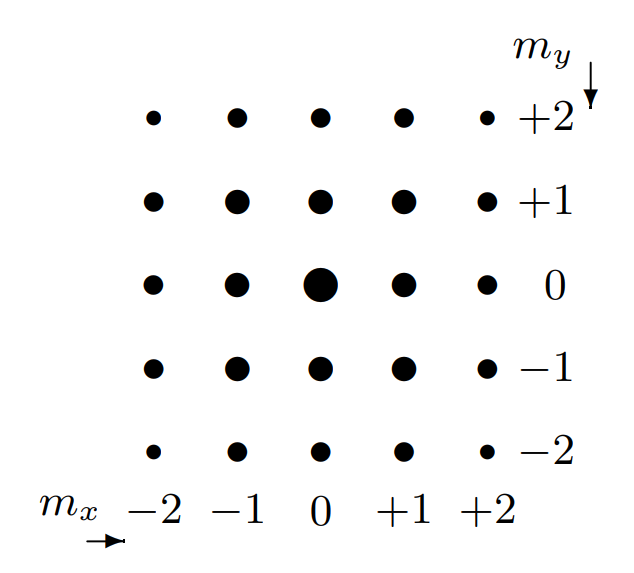
\includegraphics[width = 6cm]{4}}
	\caption{Дифракция Фраунгофера на двумерной решетке (сетке). Максимумы изображены кружками, размеры которых характеризуют интенсивности}
	\label{fig:image}
\end{figure}

Если теперь поместить в фокальной плоскости вертикальную щель так, чтобы
через нее про ходили дифракционные максимумы
с $m_x = 0$ и $m_y = 0$, $\pm 1$, $\pm 2$,..., то в плоскости
$P_2$ получится изображение решетки с горизонтально расположенными
штрихами. Если, наоборот, пропустить максимумы с $m_y = 0$ и $m_x = 0$, $\pm 1$, $\pm 2$,...,
то в $P_2$ получится изображение решетки с вертикальными штрихами.
Таким образом можно продемонстрировать явление \textsl{пространственной фильтрации} -- выделение
различных структур в изображении.

\textbf{Экспериментальная установка.} Схема модели проекционного микроскопа приведена
на рис. 5. Предметом служат сетки, расположенные в кассете. Смена сеток осуществляется поворотом внешнего
кольца кассеты.

Излучение лазера (ОКГ) почти перпендикулярно падает на сетку С, установленную вблизи фокальной плоскости линзы
Л$_1$ -- объектива микроскопа. Обычно и объектив и окуляр микроскопа -- короткофокусные
линзы (1-3 см). В нашей модели линза Л$_1$ выбирается достаточно длиннофокусной
$(f \approx 10 \text{см})$, т.к. размер первичного изображения в фокальной
плоскости $F$ должен быть не слишком малым, чтобы дополнительными диафрагмами можно было влиять на вторичное изображение
в плоскости $P_2$. Вторичное изображение из плоскости $P_2$ проецируется
на экран Э линзой Л$_2$ (короткофокусной, чтобы изображение на экране
было крупнее).

\begin{figure}[h!]
	\center{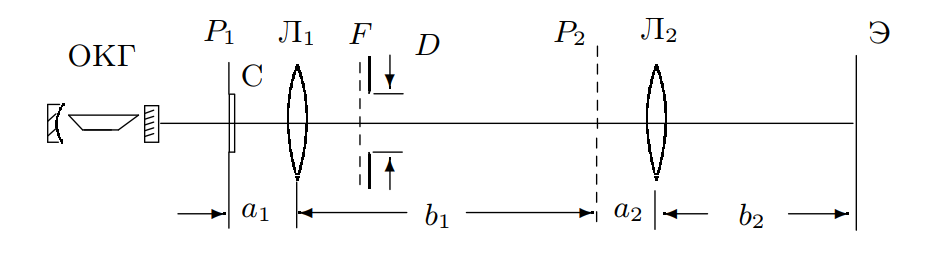
\includegraphics[width = 15cm]{5}}
	\caption{Схема экспериментальной установки -- модель проекционного микроскопа}
	\label{fig:image}
\end{figure}

Изображение сетки периодически повторяется -- \textsl{репродуцируется} --
в пространстве между сеткой и первой линзой, поэтому для того, чтобы среди множества
репродуцированных изображений сетки можно было выделить её геометрическое изображение,
на одну из сеток наложена тонкая проволочка, т.е. непериодический объект, изображение
которого не репродуцируется.

В фокальной плоскости $F$ могут быть установлены диафрагмы -- щелевая
или ирисовая (отверстие с переменным диаметром) и различного рода маски (препятствия).

Как видно из соотношения (8), минимально разрешимый шаг решетки или сетки определяется
апертурным углом $u$ объектива. Обычно апертура микроскопа меняется при помощи ирисовой диафрагмы
на объективе (на линзе Л$_1$ такая диафрагма есть), но в наших условиях удобнее располагать щелевую
диафрагму в плоскости $F$. Имея набор сеток с различными периодами $d$ и изменяя апертурный угол
объектива с помощью щелевой диафрагмы, можно экспериментально проверить соотношение (8).

В нашей работе период сеток рассчитывается двумя способами: в первом способе (дифракция Фраунгофера) --
расстояние между дифракционными максимумами на экране измеряется при помощи линейки, а затем по формуле
решетки (1) определяется ее период; во втором способе период определяется по увеличенному с помощью модели
микроскопа изображению сетки на экране.

С помощью откалиброванных таким образом сеток определяется разрешающая способность микроскопа.
Для этого в задней фокальной плоскости $F$ объектива устанавливается щелевая диафрагма с микрометрическим
винтом и подбирается ее минимальный размер, при котором еще видно изображение сетки на экране (щель пропускает
максимумы с $m = 0, \pm 1$). По размеру диафрагмы и фокусному расстоянию объектива рассчитывается апертурный угол
$u$ и проверяется соотношение (8).

Для выполнения последней части работы ширина вспомогательной щели и угол наклона к оси системы подбираются так,
чтобы на экране вместо изображения сетки получалось изображение решётки, расположенной наклонно, т.е.
осуществлялась \textsl{пространственная фильтрация}. Если сетку
и щель поменять местами, то соответствующим подбором сетки можно "рассечь" первичное изображение так, что изображение щели
на экране будет многократно повторяться -- \textsl{мультиплицироваться}.

\vspace{1cm}
\textbf{Ход работы.}

\vspace{0.5cm}
I. Измерим пространственный спектр решеток:

\begin{center}
\begin{tabular}{|c|c|c|c|c|c|c|c|c|c|}
\hline
N решетки	&	$m$		&	$mx$, мм	&	$x$, мм	&	$d$, мм	\\
\hline
1			&	6		&	215			&	35.8	&	0.02	\\
\hline
2			&	10		&	240			&	24.0	&	0.03	\\
\hline
3			&	22		&	263			&	12.0	&	0.06	\\
\hline
4			&	21		&	120			&	5.7		&	0.13	\\
\hline
5			&	11		&	45			&	4.1		&	0.18	\\
\hline
\end{tabular}
\end{center}

$d$ определим, зная расстояние $L$ от решетки до экрана: $133.0 \pm 0.2$ см. $\sigma_d$ найдем в предположении, что $d = f(x, L)$:
$$
	\sigma_d = \sqrt{\sum \left(\frac{\partial f}{\partial x_i}\sigma_{x_i}\right)^2}
$$

\vspace{1cm}
II. Определим фокусное расстояние $f = 3$ см. Также найдем расстояния $a_1, a_2, b_1, b_2$:
$$
	a_1 = 145~\text{мм},~~b_1+a_2 = 620~\text{мм},~~b_2 = 570~\text{мм}
$$
\noindent откуда, считая $a_2 = f = 30$ мм, получим
$$
	a_1 = 145~\text{мм},~~b_1 = 590~\text{мм},~~a_2 = 30~\text{мм},~~b_2 = 570~\text{мм}
$$
\noindent и, соответственно, увеличение будет равно
$$
	\frac{b_1b_2}{a_1a_2} \approx 80
$$

Измерим период увеличенного изображения сетки:

\begin{center}
\begin{tabular}{|c|c|c|c|c|c|c|c|c|c|c|c|c|c|}
\hline
N решетки	&	$m$		&	$mx$, мм	&	$x$, мм	&	$d$, мм	\\
\hline
5			&	8		&	102			&	12.8	&	0.16	\\
\hline
4			&	10		&	95			&	9.5		&	0.12	\\
\hline
3			&	16		&	75			&	4.7		&	0.06	\\
\hline
2			&	10		&	23			&	2.3		&	0.03	\\
\hline
\end{tabular}
\end{center}

Погрешность оценим, считая $d = f(x, a_1, b_1, a_2, b_2)$.

Заметим, что результаты, полученые в этом пункте, хорошо согласуются с результатами первого пункта.

\vspace{1cm}
III. Определим для каждой решётки минимальный размер диафрагмы $D$, при котором на экране еще видно изображение сетки. При этом $D = D' - D_0$, где $D'$ - прямое измерение, $D_0$ - показание винта при $D = 0$:

\begin{center}
\begin{tabular}{|c|c|c|c|c|c|c|c|c|}
\hline
N решетки	&	$d$, мм	&	$D'$, мкм	&	$D$, мкм	&	$1/D$, мкм$^{-1}\cdot 10^{-4}$	\\
\hline
5			&	0.16	&	130			&	73			&	140								\\
\hline
4			&	0.12	&	150			&	93			&	110								\\
\hline
3			&	0.06	&	215			&	158			&	60								\\
\hline
2			&	0.03	&	320			&	263 		&	40								\\
\hline
\end{tabular}
\end{center}

\begin{figure}[H]
\centering
\begin{tikzpicture}
\begin{axis}[
	height = 8cm,
	width  = 15cm,
	every axis y label/.style={at = {(ticklabel cs: 0.5)}, rotate = 90, anchor = near ticklabel},
	xlabel = {$1/D$, мкм$^{-1}\cdot 10^{-4}$},
	ylabel = {$d$, мм},
	grid   = major
]
\addplot+[
	only marks,
	error bars/.cd, 
	y dir = both, y explicit,
	x dir = both, x explicit
	]
coordinates{
	( 40, 0.03)
	( 60, 0.06)
	(110, 0.12)
	(140, 0.16)
};

\addplot [mark = none]
coordinates{
	(40, 0.031753)
	(140, 0.159641)
};

\end{axis}
\end{tikzpicture}
\captionsetup{labelformat=empty}
\caption{20}
\end{figure}

Видно, что теория Аббе выполняется. 

\newpage
Таким образом, в данной лабоаторной работе мы изучили дифракционный предел разрешения объектива микроскопа.

\end{document}
